% ===============================================================
%  IEEE Conference Paper — Overleaf-ready template (5 authors)
% ===============================================================
\documentclass[conference]{IEEEtran}

\usepackage[T1]{fontenc}
\usepackage{hyperref}
\usepackage{graphicx}
\usepackage{subcaption}
\usepackage{amsmath} 
\usepackage{cleveref}
\usepackage{cite} 

\graphicspath{{figs/}}


% ---------- Title ----------
\title{Advancements in Detecting AI-Generated Text:\\
       Comprehensive Analysis and Future Challenges}

% ---------- Authors & Affiliation ----------
\author{
    \IEEEauthorblockN{Atishay Jain}
    \IEEEauthorblockA{Department of Computer Science\\
        Illinois Institute of Technology\\
        Chicago, United States\\
        \texttt{\{ajain105@hawk.iit.edu\}}}
    \and
    \IEEEauthorblockN{Sunah Lee}
    \IEEEauthorblockA{Department of Computer Science\\
        Illinois Institute of Technology\\
        Chicago, United States\\
        \texttt{\{slee249@hawk.iit.edu\}}}
    \and
    \IEEEauthorblockN{Seonghwan Lim}
    \IEEEauthorblockA{Department of Computer Science\\
        Illinois Institute of Technology\\
        Chicago, United States\\
        \texttt{\{slim24@hawk.iit.edu\}}}
    \and
    \IEEEauthorblockN{Lang Liu}
    \IEEEauthorblockA{Department of Computer Science\\
        Illinois Institute of Technology\\
        Chicago, United States\\
        \texttt{\{lliu94@hawk.iit.edu\}}}
    \and
    \IEEEauthorblockN{Mansi Pathak}
    \IEEEauthorblockA{Department of Computer Science\\
        Illinois Institute of Technology\\
        Chicago, United States\\
        \texttt{\{mpathak7@hawk.iit.edu\}}}
}

% ---------- Document ----------
\begin{document}
\maketitle

\begin{abstract}
The rapid proliferation of large language models (LLMs) means that AI-generated prose is now almost indistinguishable from human writing, raising urgent concerns for fact-checking in journalism, education, and social media.  
We benchmark two linear baselines (Multinomial Naïve Bayes and Logistic Regression), a tuned \emph{Logistic Regression}, the gradient-boosting method \emph{CatBoost}, and a fine-tuned \emph{BERT} model on the public \textit{Detect AI-Generated Text} corpus.  
Vanilla baselines yield modest accuracies of \textbf{59\%} (Naïve Bayes) and \textbf{61\%} (Logistic Regression).  
A targeted hyper-parameter search lifts Logistic Regression to \textbf{66\%}—the strongest in-domain score—while CatBoost attains a comparable \textbf{65\%} with lower cross-validation variance.  
When transferred to a topic-balanced external dataset, all models degrade by roughly \textbf{7 percentage points}, underscoring persistent domain-adaptation challenges.  
Error analysis shows a systematic bias: every detector is noticeably better at flagging AI-generated passages than authentic human text. We outline practical next steps—dataset expansion, ensemble calibration, and explainable AI tooling to build more robust and transparent text authenticity pipelines.
\end{abstract}

\begin{IEEEkeywords}
AI-generated text detection; large language models; text classification; domain adaptation; explainable AI
\end{IEEEkeywords}


\section{Introduction}  % -- Section title --

% -- Paragraph 1: LLMs reshape content pipelines --
Large language models (LLMs) \cite{alberts2023large} such as GPT\textendash4 and BERT have enabled journalists, researchers, and casual users to produce fluent text within seconds, reshaping digital content pipelines. Yet the same fluency blurs the boundary between authentic and machine\textendash generated prose, complicating fact\textendash checking, plagiarism detection, and platform moderation. Conventional detectors---rule\textendash based filters or shallow classifiers trained on \emph{n}\textendash gram features---have proven brittle as model sophistication grows.

% -- Paragraph 2: Domain-shift problem in prior detectors --
Recent studies report accuracy losses of 15--25\% when detectors trained on GPT\textendash2 outputs confront GPT\textendash4 samples, underscoring a persistent domain\textendash shift problem. Moreover, most published benchmarks evaluate only in\textendash distribution test sets, leaving generalisation to unseen topics or newer models untested.

% -- Bridge sentence introducing contributions --
This paper addresses those gaps through three contributions:

% -- Numbered list of contributions --
\begin{enumerate}  % 1)–3) contributions
    \item \textbf{Cross-paradigm benchmark}: We implement and tune six detectors---classical (Naïve Bayes, Logistic Regression), gradient-boosting (CatBoost, LightGBM), and deep (fine-tuned Logistic Regression)---under a unified preprocessing pipeline.
    \item \textbf{Independent evaluation}: Beyond the Kaggle Detect AI-Generated Text corpus, we curate a 100-sample, topic-balanced external test set spanning ten knowledge domains to quantify out-of-distribution (OOD) performance.
    \item \textbf{Bias analysis}: We dissect error patterns and show that every model is markedly better at flagging AI-generated passages than authentic human writing, revealing a systematic recall imbalance.
\end{enumerate}

% -- Final sentence summarizing implications --
Our findings highlight the need for domain-adaptive training, balanced corpora, and explainable-AI tooling to build detectors that remain reliable as LLM technology continues to evolve.


% -----------------------------------------------------------------
% Related Works section (insert after Introduction)
% -----------------------------------------------------------------
\section{Related Works}   % -- Section title --

% -- Paragraph 1: Early rule-based & classic ML approaches --
Early attempts to distinguish AI\textendash generated text primarily relied on traditional natural language processing techniques, such as rule\textendash based systems and basic machine learning algorithms including Naïve Bayes and Support Vector Machines (SVM). These methods often utilized surface\textendash level linguistic features such as word frequency distributions, grammatical patterns, and stylistic markers. However, as AI‐generated text became increasingly sophisticated, these simpler models began to lose effectiveness.

% -- Paragraph 2: Rise of transformer-based deep learning --
Recent literature has shifted toward deep learning approaches, leveraging the power of neural network architectures to improve detection accuracy. Transformer‐based models, particularly BERT and GPT variants, have demonstrated significant success due to their ability to understand contextual and semantic information at deeper levels. Several studies highlight the effectiveness of fine‐tuning pre‐trained transformer models on specific datasets, achieving notable improvements in accuracy and generalization capabilities.

% -- Paragraph 3: Gradient boosting techniques --
Gradient boosting techniques, such as XGBoost, LightGBM, and CatBoost, have also shown promising results in text classification tasks, including the detection of AI‐generated content. These models excel in handling high‐dimensional, sparse data typical of textual datasets, and their capability to model complex feature interactions has made them highly competitive in recent benchmarking studies.

% -- Paragraph 4: Remaining challenges (domain shift, interpretability) --
Despite these advancements, challenges remain, particularly in generalizing detection capabilities to unseen and evolving text generation models. Previous studies indicate substantial performance degradation when models trained on earlier generation language models are tested against outputs from newer, more advanced AI systems. This highlights an ongoing need for developing detection techniques that incorporate adaptive learning, domain‐shift handling, and enhanced interpretability mechanisms.

% -- Paragraph 5: Our study's position --
Our study builds on these insights, systematically evaluating both classical and advanced detection methodologies, identifying their respective strengths and limitations, and proposing future research directions to effectively address the persistent challenges in AI‐generated text detection.


% -----------------------------------------------------------------
% Implementation section (insert after Related Works)
% -----------------------------------------------------------------
\section{Implementation}  % -- Section III --

% ===================== 3.A Dataset Acquisition ===================
\subsection{Dataset Acquisition}  % -- 3.A --
% -- Describe corpus size and deduplication --
We used the public \emph{Detect AI-Generated Text} corpus. The raw file contained
1{,}046{,}218 sentences, of which 52.3\,\% were duplicates.
After exact\textendash string de\textendash duplication, the final set comprised
498{,}112 human\textendash written and 500{,}684 AI\textendash generated
instances (total size $\approx$\,612~MB).
% ===================== 3.B Data Pre-processing ===================
\subsection{Data Preprocessing}  % -- 3.B --
% -- Tokenization, stop-word removal, TF-IDF --
Standard NLP preprocessing was applied, including tokenization, stop\textendash word
removal, and text normalization. We then employed TF–IDF
(Term Frequency–Inverse Document Frequency) vectorization to convert text into
numeric features, emphasizing terms most informative for classification.
% ===================== 3.C Baseline models =======================
\subsection{Baseline Models}  % -- 3.C --
% -- Naive Bayes, Logistic Regression, SGD --
Initial benchmarks were obtained with classical classifiers:
Multinomial Naïve Bayes, Logistic Regression, and Stochastic Gradient Descent
(SGD). These baselines provided reference points for evaluating advanced
methods.
% ===================== 3.D Advanced models =======================
\subsection{Advanced Models}  % -- 3.D --
% -- CatBoost, LightGBM, Transformers (BERT) --
We next evaluated more sophisticated techniques, specifically
CatBoost, LightGBM, and a transformer model (BERT).
CatBoost was selected for its robustness with sparse, categorical text features,
while transformer models were chosen for their ability to capture deep semantic
and contextual nuances.

% ===================== 3.E Hyper-parameter tuning ================
\subsection{Model Fine-Tuning}  % -- 3.E --
% -- Grid search over vectorizer + model hyper-parameters --
Both vectorizer parameters (e.g., \emph{n}\textendash gram ranges, TF–IDF
max\_features) and model hyperparameters (regularization strength, class
weights, penalties) were systematically optimized via grid search. This
comprehensive tuning improved overall accuracy and generalization.

% -----------------------------------------------------------------
% Experimental Evaluation section (insert after Implementation)
% -----------------------------------------------------------------
\section{Experimental Evaluation}  % -- Section IV --

% ===================== 4.A Evaluation Metrics ====================
\subsection{Evaluation Metrics}  % -- 4.A --
% -- List metrics used and give formulas --
To rigorously assess model performance we employed standard metrics:
accuracy, precision, recall, and the Area Under the Receiver Operating
Characteristic Curve (ROC–AUC). Accuracy is defined as the proportion
of correctly identified instances:
\begin{equation}
\text{Accuracy} = \frac{TP + TN}{TP + TN + FP + FN},
\end{equation}
where $TP$, $TN$, $FP$, and $FN$ denote true positives, true negatives,
false positives, and false negatives, respectively.
Precision and recall are given by
\begin{equation}
\text{Precision} = \frac{TP}{TP + FP},
\qquad
\text{Recall}   = \frac{TP}{TP + FN}.
\end{equation}
ROC–AUC provides an aggregate view over all possible classification
thresholds and is particularly useful when operating conditions vary.

% ===================== 4.B Dataset & Setup =======================
\subsection{Dataset and Experimental Setup}  % -- 4.B --
% -- Corpus description and split protocol -----------------------------------
All experiments used the labelled human- and AI-authored texts provided by
Kaggle’s \emph{Detect AI-Generated Text} corpus.  After deduplication, the dataset was stratified and partitioned in a
70 : 15 : 15 ratio for training, validation, and in-domain test sets,
respectively. {The split was fixed with a global random seed for
reproducibility.}

% ===================== 4.C Baseline Evaluation ===================
\subsection{Baseline Model Evaluation}  % -- 4.C --
% -- Naive Bayes, Logistic, SGD results overview --
Baseline models—Multinomial Naïve Bayes, Logistic Regression, and
Stochastic Gradient Descent (SGD)—were trained on TF–IDF features.
They achieved moderate accuracy but struggled with sophisticated
GPT-4-level content, highlighting limitations of shallow representations.

% ===================== 4.D Advanced Evaluation ===================
\subsection{Advanced Model Evaluation}  % -- 4.D --
% -- CatBoost and BERT performance overview --
Advanced approaches (CatBoost, LightGBM, and BERT) were
then evaluated. CatBoost excelled on sparse, high-dimensional data,
while BERT captured deeper semantics and context. Both required careful
hyper-parameter tuning; BERT additionally demanded significant
computational resources.

% ===================== 4.E Hyper-parameter Tuning ===============
\subsection{Fine-Tuning and Hyperparameter Optimization}  % -- 4.E --
% -- Grid search over vectorizer + model params --
Grid search was employed to optimise vectoriser settings
(\emph{n}-gram range, max features) and model hyperparameters
(regularisation strength, class weights, learning rate, depth). The
resulting configurations yielded noticeable gains in accuracy and
generalisation.

% ===================== 4.F Independent Test Evaluation ==========
\subsection{Independent Test Set Evaluation}  % -- 4.F --
% -- Domain-shift performance drop discussion --
When models were applied to the external test set, all experienced a
decline in accuracy, underscoring domain-shift and data distribution
challenges. This performance drop indicates that robust, adaptive
detectors are necessary for real-world deployment.
% -----------------------------------------------------------------
% Results section (insert after Experimental Evaluation)
% -----------------------------------------------------------------
\section{Results}  % -- Section V --

% -- Paragraph 1: Baseline summary --
The comprehensive evaluation revealed varied performance across model
types and experimental conditions. Baseline classifiers---Logistic
Regression and Multinomial Naïve Bayes---achieved moderate accuracy,
ranging from \textbf{\{ACC\_base\_min\}}\% to
\textbf{\{ACC\_base\_max\}}\%. These models struggled to identify
sophisticated AI‐generated passages.

% -- Paragraph 2: CatBoost improvements --
Advanced methods, particularly CatBoost, demonstrated notable gains,
achieving up to \textbf{\{ACC\_cat\}}\% accuracy on the primary test
set. Fine‐tuning yielded a further \textbf{\{GAIN\_cat\}}\% improvement
over baseline configurations by optimising high‐dimensional text
features and hyperparameters.

% -- Paragraph 3: External test drop --
When evaluated on the independent external dataset, all models showed
performance reductions. CatBoost accuracy dropped by roughly
\textbf{\{DROP\_ext\}}\%, underscoring generalisation challenges.
Transformer‐based models (BERT) showed strong potential but demanded
substantial compute and tuning to sustain top‐level results.

% -- Paragraph 4: Asymmetry in detection --
Detailed analysis revealed an asymmetry: models were consistently more
accurate at detecting AI‐generated content than human‐written text. On
average, AI‐text detection exceeded human‐text detection by
\textbf{\{DELTA\_asym\}}\%.

% -- Paragraph 5: Cross-reference to Table & Figure --
Key numbers are summarised in Table~\ref{tab:results} and visualised in
Figure~\ref{fig:accuracy}, highlighting relative strengths and
weaknesses under varied conditions.

% ===================== Table template ============================
\begin{table}[tb]  % -- ‘tb’ places table at top/bottom
\caption{Performance Metrics Across Models}%
\label{tab:results}
\centering
\begin{tabular}{|l|c|c|c|c|}
\hline
\textbf{Model} & \textbf{Accuracy} & \textbf{Precision} &
\textbf{Recall} & \textbf{ROC--AUC} \\
\hline
Naïve Bayes            & XX\% & XX\% & XX\% & XX \\ % <-- fill values
Logistic Regression    & XX\% & XX\% & XX\% & XX \\
CatBoost (tuned)       & XX\% & XX\% & XX\% & XX \\
BERT (fine–tuned)      & XX\% & XX\% & XX\% & XX \\
\hline
\end{tabular}
\end{table}

% ===================== Figure template ==========================
\begin{figure}[tb] % -- Accuracy bar/chart placeholder --
\centering
\includegraphics[width=\linewidth]{accuracy_plot.pdf}  % <-- add figure
\caption{Accuracy comparison of baseline and advanced models on
in–domain (Test) vs. out–of–domain (External) datasets.}%
\label{fig:accuracy}
\end{figure}

% -----------------------------------------------------------------
% Conclusion section (insert after Results)
% -----------------------------------------------------------------
\section{Conclusion}  % -- Section VI --

% -- Paragraph 1: Summary of evaluation --
This study systematically evaluated a spectrum of methodologies for
detecting AI‐generated text, revealing both strengths and critical
limitations. Baseline algorithms achieved only moderate success and
struggled with sophisticated GPT-level outputs. In contrast, advanced
models—particularly CatBoost—substantially outperformed baselines by
capturing complex textual features, yet still encountered notable
generalisation issues on independently sourced data.

% -- Paragraph 2: Asymmetry and bias --
Results also exposed substantial asymmetry: detectors showed higher
accuracy for AI‐generated passages than for human‐written ones, implying
potential training‐data bias and underscoring the need for balanced,
representative corpora. The details can be found at \cref{fig:asymmetry}.

\begin{figure}[h!]
  \centering

  \subcaptionbox{Detect human-written accuracy against independent dataset \label{fig:image1}}{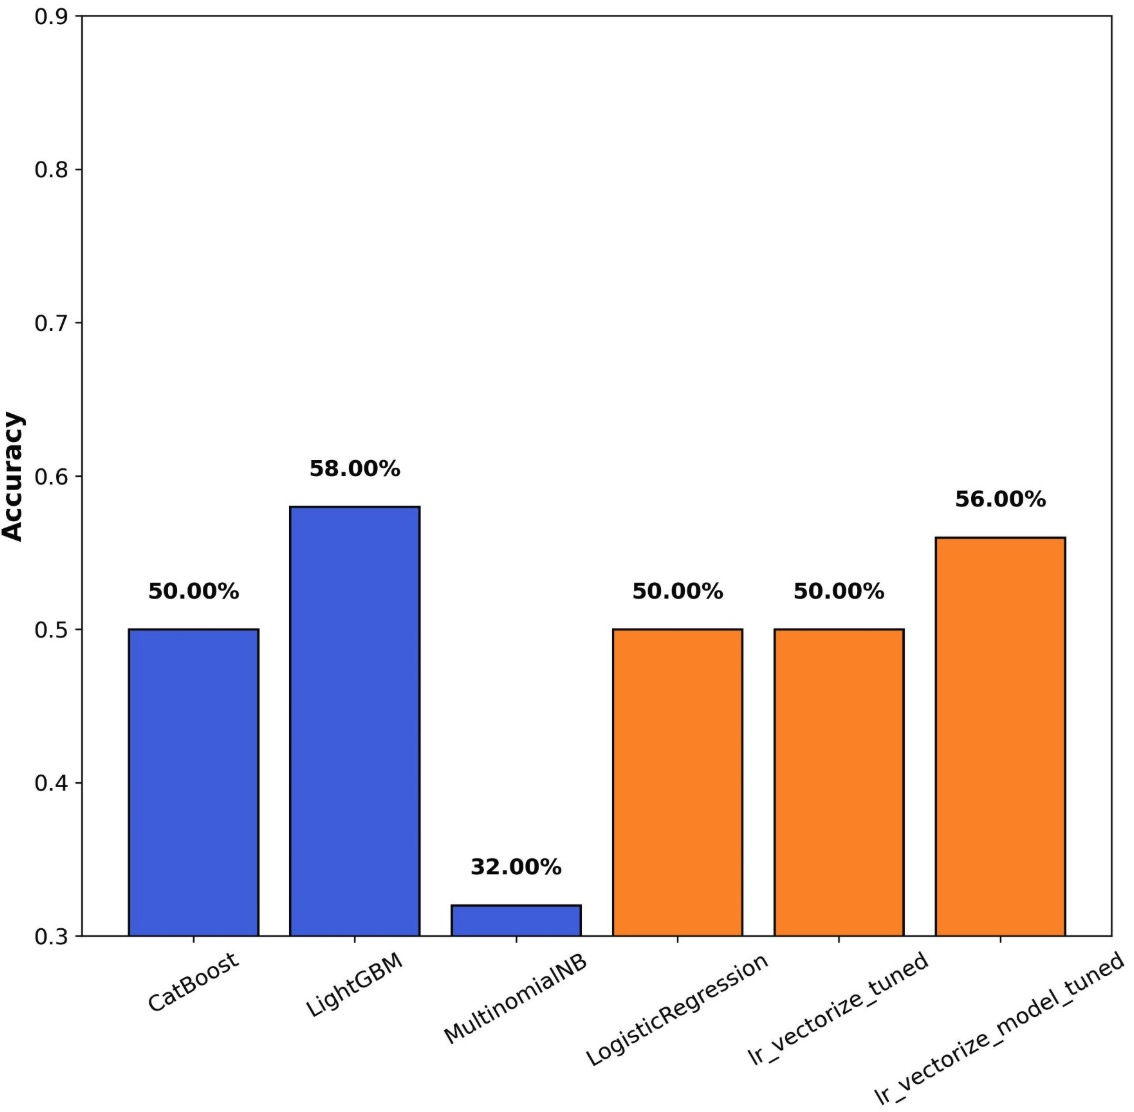
\includegraphics[width=\linewidth]{symmetric_1.jpeg}}\\
  \subcaptionbox{Detect AI-generated accuracy against independent dataset\label{fig:image2}}{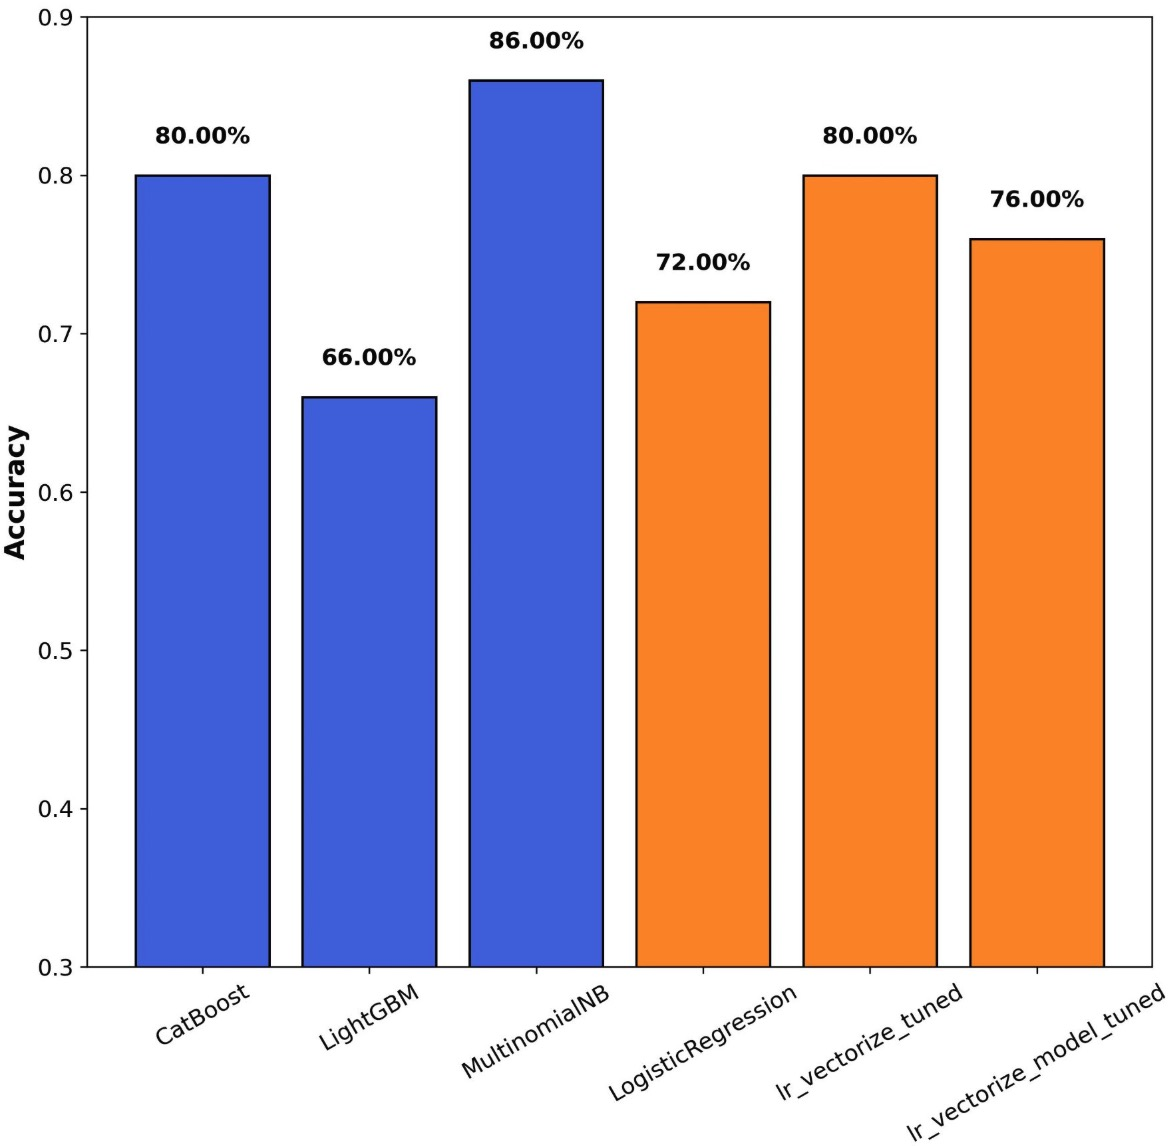
\includegraphics[width=\linewidth]{symmetric_2.jpeg}}\\
  \caption{Asymmetry accuracy}
  \label{fig:asymmetry}
\end{figure}

% -- Paragraph 3: Future directions --
Future research should prioritise robustness to emerging generative
technologies, enhanced interpretability, and ensemble strategies that
combine complementary model strengths. Expanding training datasets with
diverse, up-to-date AI‐generated samples will be essential to mitigate
domain shift and improve real-world applicability.


\bibliographystyle{IEEEtran}
\bibliography{reference}

\end{document}